\section{Développement firmware} \label{sec:Dev-firmware}

Lors de cette section, nous décrirons le processus de développement du firmware du PIC32. Les décisions prises seront expliquées et les différents algorithmes seront illustrés et décrits.

En premier lieux nous allons analyser lors de la section \ref{ssec:ProtocolGNSS} comment traiter les données du \gls{gnss}, il s'agit d'un élément critique.


\subsection{Protocoles du GNSS} \label{ssec:ProtocolGNSS}
Il existe différents protocoles pour le format de données de localisation. Le \textbf{CAM-M8C-0} supporte plusieurs protocoles, visibles sur la figure \ref{fig:protocolsGNSS} :

\begin{figure}[h]
	\centering
	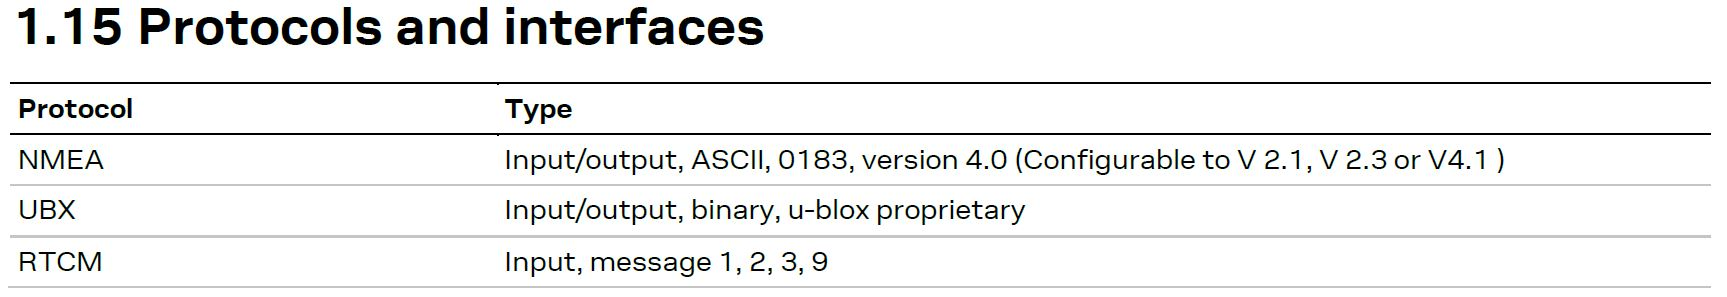
\includegraphics[width=.75\linewidth]{../figures/code/Protocols}
	\caption{Protocoles disponibles.}
	\source{\Gls{datasheet} du \href{https://content.u-blox.com/sites/default/files/CAM-M8-FW3\_DataSheet\_\%28UBX-15031574\%29.pdf}{CAM-M8C-0}}
	\label{fig:protocolsGNSS}
\end{figure} \vspace{-4mm}

\begin{tabularx}{\textwidth}{llX}
	\textbf{NMEA}& : & Norme établie par la \textit{National Marine Electronics Association}. Elle suit un format \fbox{\textbf{ASCII}}. \\
	\textbf{UBX} & : & Format propriétaire de u-blox avec des données \fbox{\textbf{binaires}}. Il permet d'envoyer des trames de configuration. \\
	\textbf{RTCM} & : & Protocole pour des données GPS différentielles. Établi par la \textit{Radio Technical Commission for Maritime Service}.
\end{tabularx} 


Le \textbf{CAM-M8C-0} est configuré, par défaut, pour envoyer des messages au format NMEA, comme illustré sur la figure \ref{fig:default-messages}. \vspace{+2mm}

\begin{figure}[!h]
	\centering
	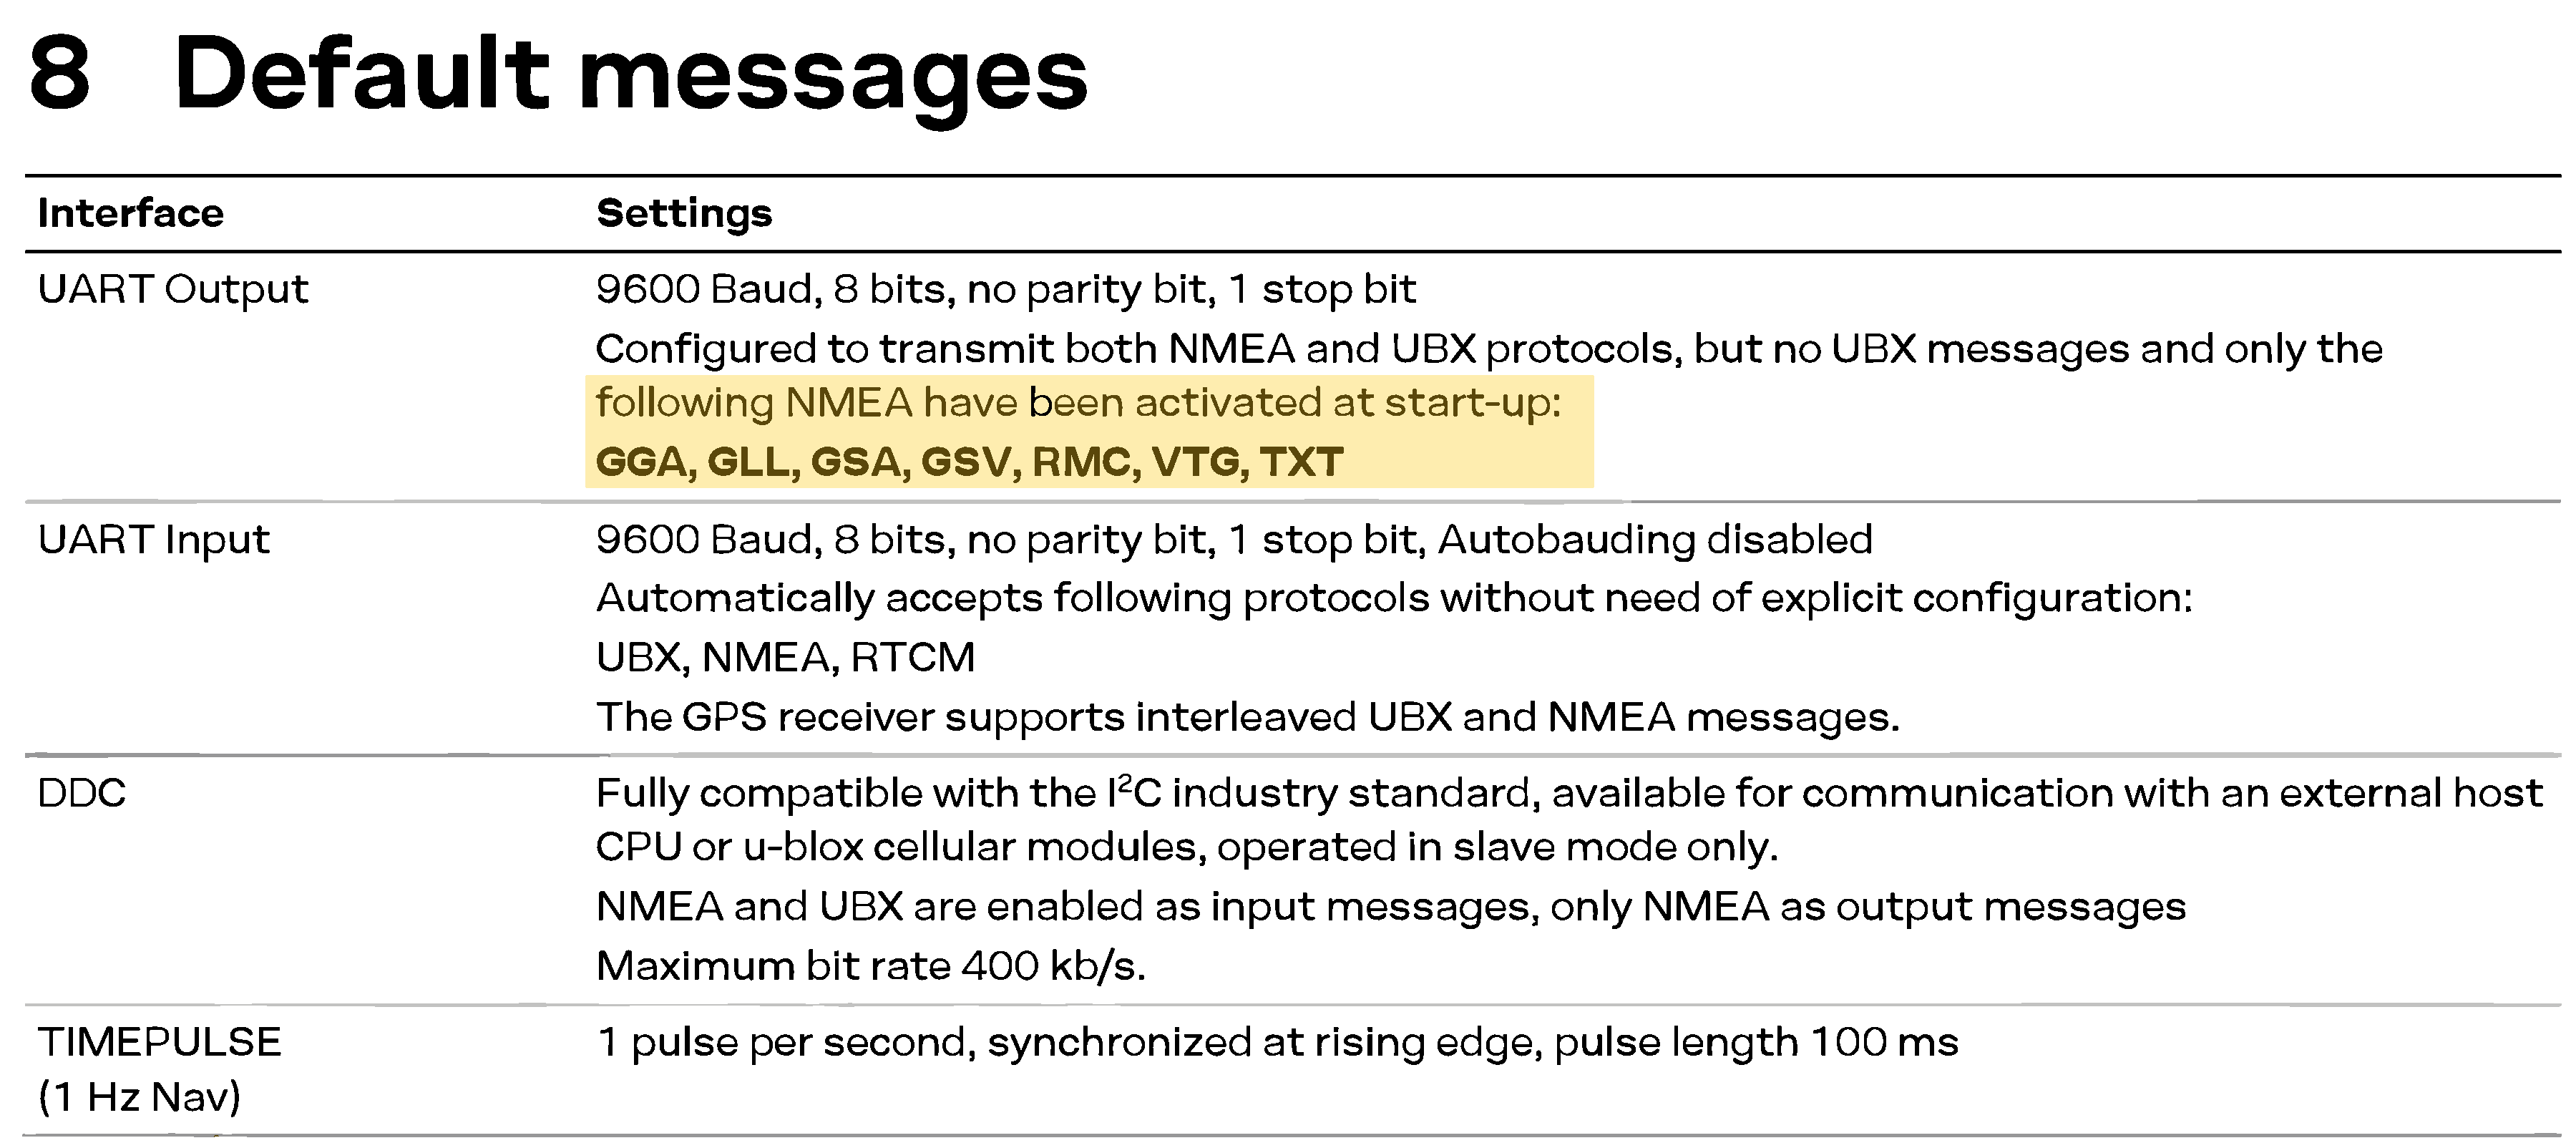
\includegraphics[width=0.7\linewidth]{../figures/code/Default-messages}
	\caption{Protocole par défaut.}
	\source{\Gls{datasheet} du \href{https://content.u-blox.com/sites/default/files/CAM-M8-FW3\_DataSheet\_\%28UBX-15031574\%29.pdf}{CAM-M8C-0}}
	\label{fig:default-messages}
\end{figure}

\clearpage

\subsubsection{Messages NMEA}
Comme nous avons pu constater sur la figure \ref{fig:default-messages}, il y a plusieurs messages \textbf{NMEA} : 

\textbf{GGA, GLL, GSA, GSV, RMC, VTG, TXT}

Ceux-ci sont décris dans le \href{https://www.ekf.de/c/cgps/cg2/inf/nmea_reference_manual.pdf}{manuel de référence du protocole NMEA} sur la figure \ref{fig:messages-nmea}

\begin{figure}[h]
	\centering
	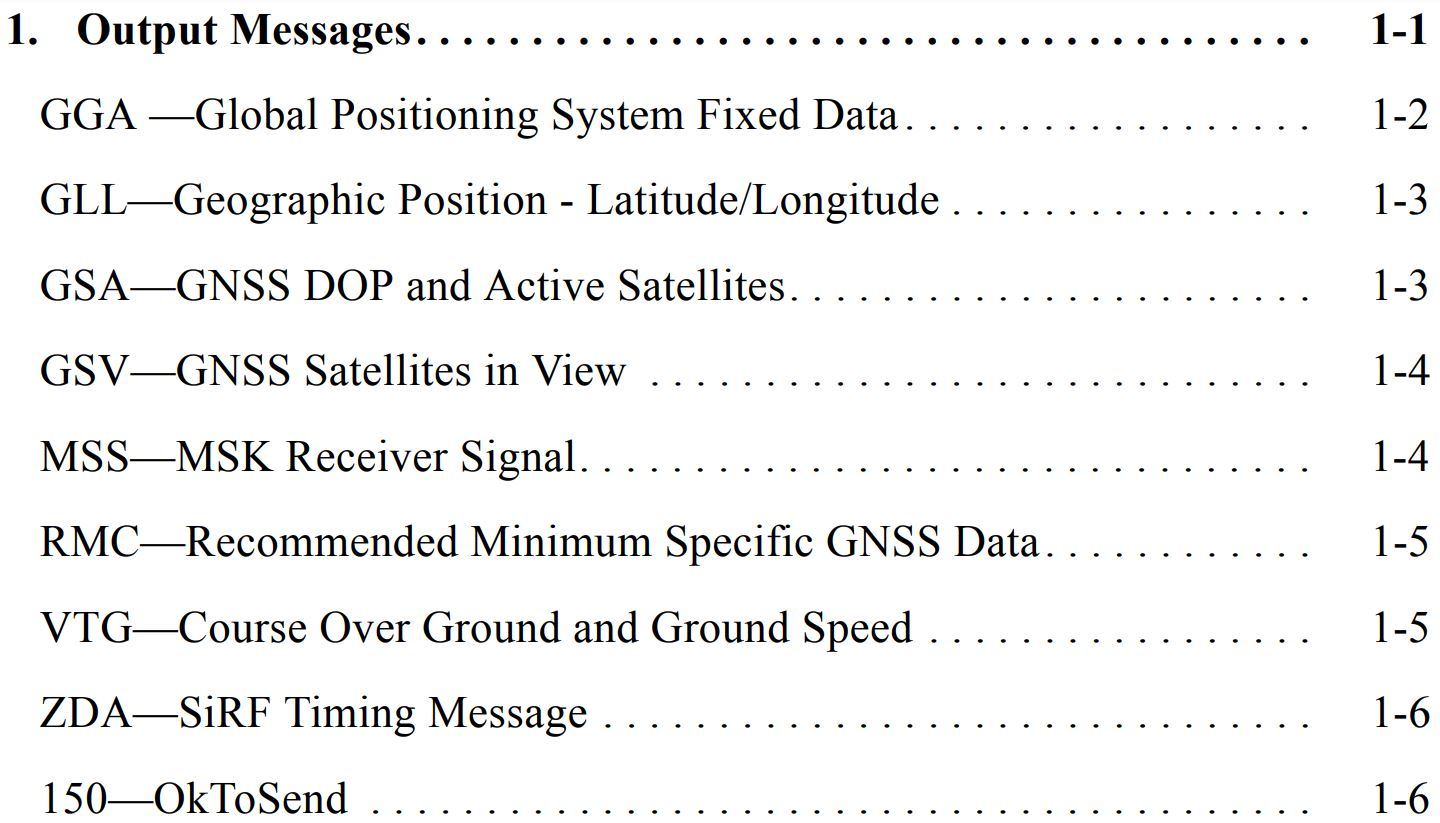
\includegraphics[width=0.55\linewidth]{../figures/code/Messages-NMEA}
	\caption{Messages NMEA.}
	\source{\href{https://www.ekf.de/c/cgps/cg2/inf/nmea_reference_manual.pdf}{Manuel du protocole NMEA}}
	\label{fig:messages-nmea}
\end{figure}

Les différents messages de la figure \ref{fig:messages-nmea} présentent des différentes données sous divers formats. Les messages peuvent être activés ou désactivés en configurant le module u-blox.

\subsubsection{Interprétation des données NMEA}
Avant d'avoir le \gls{pcb} monté et exploitable, sachant que nous connaissons le protocole par défaut du module, nous pouvons analyser des données \textbf{NMEA} pour mieux les comprendre et les traiter par la suite. Pour ce faire, le site \href{https://www.nmeagen.org/}{https://www.nmeagen.org/} permet de générer des coordonnées avec le protocole \textbf{NMEA}.

\begin{figure}[h]
	\centering
	\includegraphics[width=.75\textwidth]{../figures/code/map-localisation}
	\caption{Application d'une localisation NMEA.}
	\source{\href{https://www.nmeagen.org/}{nmeagen.org}, aéroport de La Blécherette, Lausanne}
	\label{fig:map-localisation}
\end{figure}

Sur la figure \ref{fig:parsed-nmea}, les messages de la figure \ref{fig:map-localisation} sont décodés via un \href{https://swairlearn.bluecover.pt/nmea_analyser}{analyseur NMEA en ligne}.

\begin{figure}[h]
	\centering
	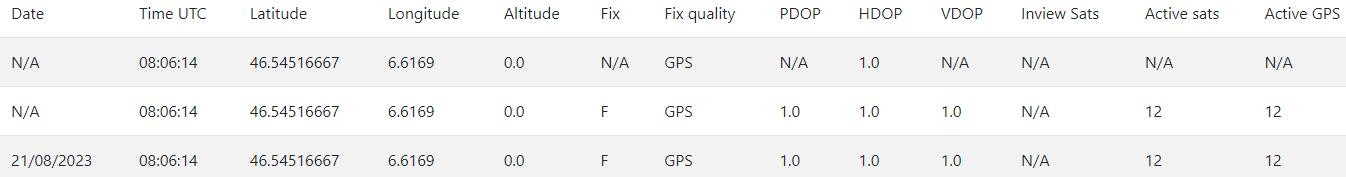
\includegraphics[width=0.8\linewidth]{../figures/code/parsed-nmea}
	\caption{Messages NMEA décodés.}
	\source{\href{https://swairlearn.bluecover.pt/nmea_analyser}{NMEA online analyser}}
	\label{fig:parsed-nmea}
\end{figure}

\clearpage

\subsubsection{Code décodeur de trame NMEA}
Afin de développer le code du décodeur \textbf{NMEA}, la librairie \href{https://github.com/kosma/minmea}{\textbf{minmea}} de licence libre, a pu être utilisée, modifiée et adaptée. Un algorithme a ensuite été mis en place :

\begin{itemize}
	\item[\oldstylenums{1}] Lecture du type de message (\textbf{GBS, GGA, GLL, GSA, GST, GSV, RMC, VTG, ZDA});
	\item[\oldstylenums{2}] Parsing des valeurs correspondantes à l'ID du message;
	\item[\oldstylenums{3}] Sauvegarde des valeurs dans une structure.
\end{itemize}


\begin{code}
\caption{gnss\_posGet\_nmea(...), décodage \textbf{NMEA}.}
\label{code:posget-nmea}
\begin{minted}[breaklines]{c}
// Get message ID, strict
*msg_id = minmea_sentence_id(message, true);
// Parse message depending on ID
if (*msg_id == MINMEA_SENTENCE_GBS)
	minmea_parse_gbs(&sentences->gbs, message);
else if (*msg_id == MINMEA_SENTENCE_GGA)
	minmea_parse_gga(&sentences->gga, message);
else if ...
\end{minted}
\end{code}

Dans le code \ref{code:posget-nmea}, on fait appel à une fonction qui va masquer les caractères du type du message. Ensuite, selon le message dont il s'agit, on le décode de différentes façons.

\begin{code}
\caption{minmea\_parse\_gbs(...), décodage message \textbf{GBS}.}
\label{code:parse-gbs}
\begin{minted}[breaklines]{c}
bool minmea_parse_gbs(struct minmea_sentence_gbs *frame, const char *sentence)
{
	// $GNGBS,170556.00,3.0,2.9,8.3,,,,*5C
	char type[6];
	if (!minmea_scan(sentence, "tTfffifff",
			type,
			&frame->time,
			&frame->err_latitude,
			&frame->err_longitude,
			&frame->err_altitude,
			&frame->svid,
			&frame->prob,
			&frame->bias,
			&frame->stddev
			))
		return false;
	if (strcmp(type+2, "GBS"))
		return false;
	return true;
}
\end{minted}
\end{code}

Dans le code \ref{code:parse-gbs}, on masque les éléments du message selon son format, d'une manière similaire à la fonction standard \textit{\textbf{scanf(...)}}.

\clearpage

Les données spécifique au message \textbf{GBS} sont ensuite stockées dans une structure, que l'on peut observer dans le code \ref{code:struct-gbs}.

\begin{code}
\caption{Structure \textbf{GBS}.}
\label{code:struct-gbs}
\begin{minted}[breaklines]{c}
struct minmea_sentence_gbs {
	struct minmea_time time;
	struct minmea_float err_latitude;
	struct minmea_float err_longitude;
	struct minmea_float err_altitude;
	int svid;
	struct minmea_float prob;
	struct minmea_float bias;
	struct minmea_float stddev;
};
\end{minted}
\end{code}

Sachant que plusieurs types de messages peuvent être interceptés, chacune des structures des différents formats de messages est elle-même stockée dans une structure que l'on peut observer dans le code \ref{code:struct-msgs}.

\begin{code}
\caption{Structures messages.}
\label{code:struct-msgs}
\begin{minted}[breaklines]{c}
typedef struct minmea_messages{
	struct minmea_sentence_gbs gbs;
	struct minmea_sentence_rmc rmc;
	struct minmea_sentence_gga gga;
	struct minmea_sentence_gll gll;
	struct minmea_sentence_gst gst;
	struct minmea_sentence_gsa gsa;
	struct minmea_sentence_gsv gsv;
	struct minmea_sentence_vtg vtg;
	struct minmea_sentence_zda zda;
}minmea_messages;
\end{minted}
\end{code}

Les données sont ensuite traitées dans l'application. Pour paramétrer le \textbf{CAM-M8C-0}, des messages \textbf{UBX} peuvent être envoyés. Pour ce faire, des éléments de la librairie \href{https://github.com/u-blox/ubxlib}{\textit{ubxlib}} peuvent être repris, notamment les fonctions d'encodage et de décodage des messages \textbf{UBX}.



\subsection{Configuration des périphériques}
Les périphériques utilisés par le microcontrôleur doivent êtres paramétrés et initialisés. Le configurateur \gls{harmony} permet de le faire simplement.

\begin{figure}[h]
	\centering
	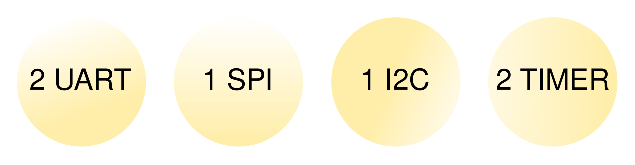
\includegraphics[width=.5\linewidth]{../figures/code/périphériques}
\end{figure}

\clearpage

\subsubsection{Timers}
Lors de cette section, 2 timers vont être configurés, ceux-ci ont des utilités différentes :

\begin{table}[h]
\begin{tabular}{lll}
	\textbf{Timer 1} & sert pour les attentes bloquantes précises. & 1 [$ms$] \\
	\textbf{Timer 2} & gère les délais entre les mesures et l'affichage des LEDs. & 10 [$ms$] \\
\end{tabular} 
\end{table} \vspace*{-5pt}

\underline{Dimensionnement timer 1}

$f_{sys} = 72\;MHz$

$f_{per} = 1\;kHz$

$presc = 8\;[-]$ \vspace*{-5pt}

\begin{equation*}
	C_{T1} = \frac{f_{sys}}{f_{per}*presc} - 1 = \frac{72*10^{6}}{1*10^{3}*8} - 1 = 8'999\; [-]
\end{equation*}


\underline{Dimensionnement timer 2}

$f_{sys} = 72\;MHz$

$f_{per} = 100\;Hz$

$presc = 16\;[-]$ \vspace*{-5pt}

\begin{equation}
	C_{T1} = \frac{f_{sys}}{f_{per}*presc} - 1 = \frac{72*10^{6}}{100*16} - 1 = 44'999\; [-]
\end{equation}

\begin{figure}[h]
	\centering
	\fbox{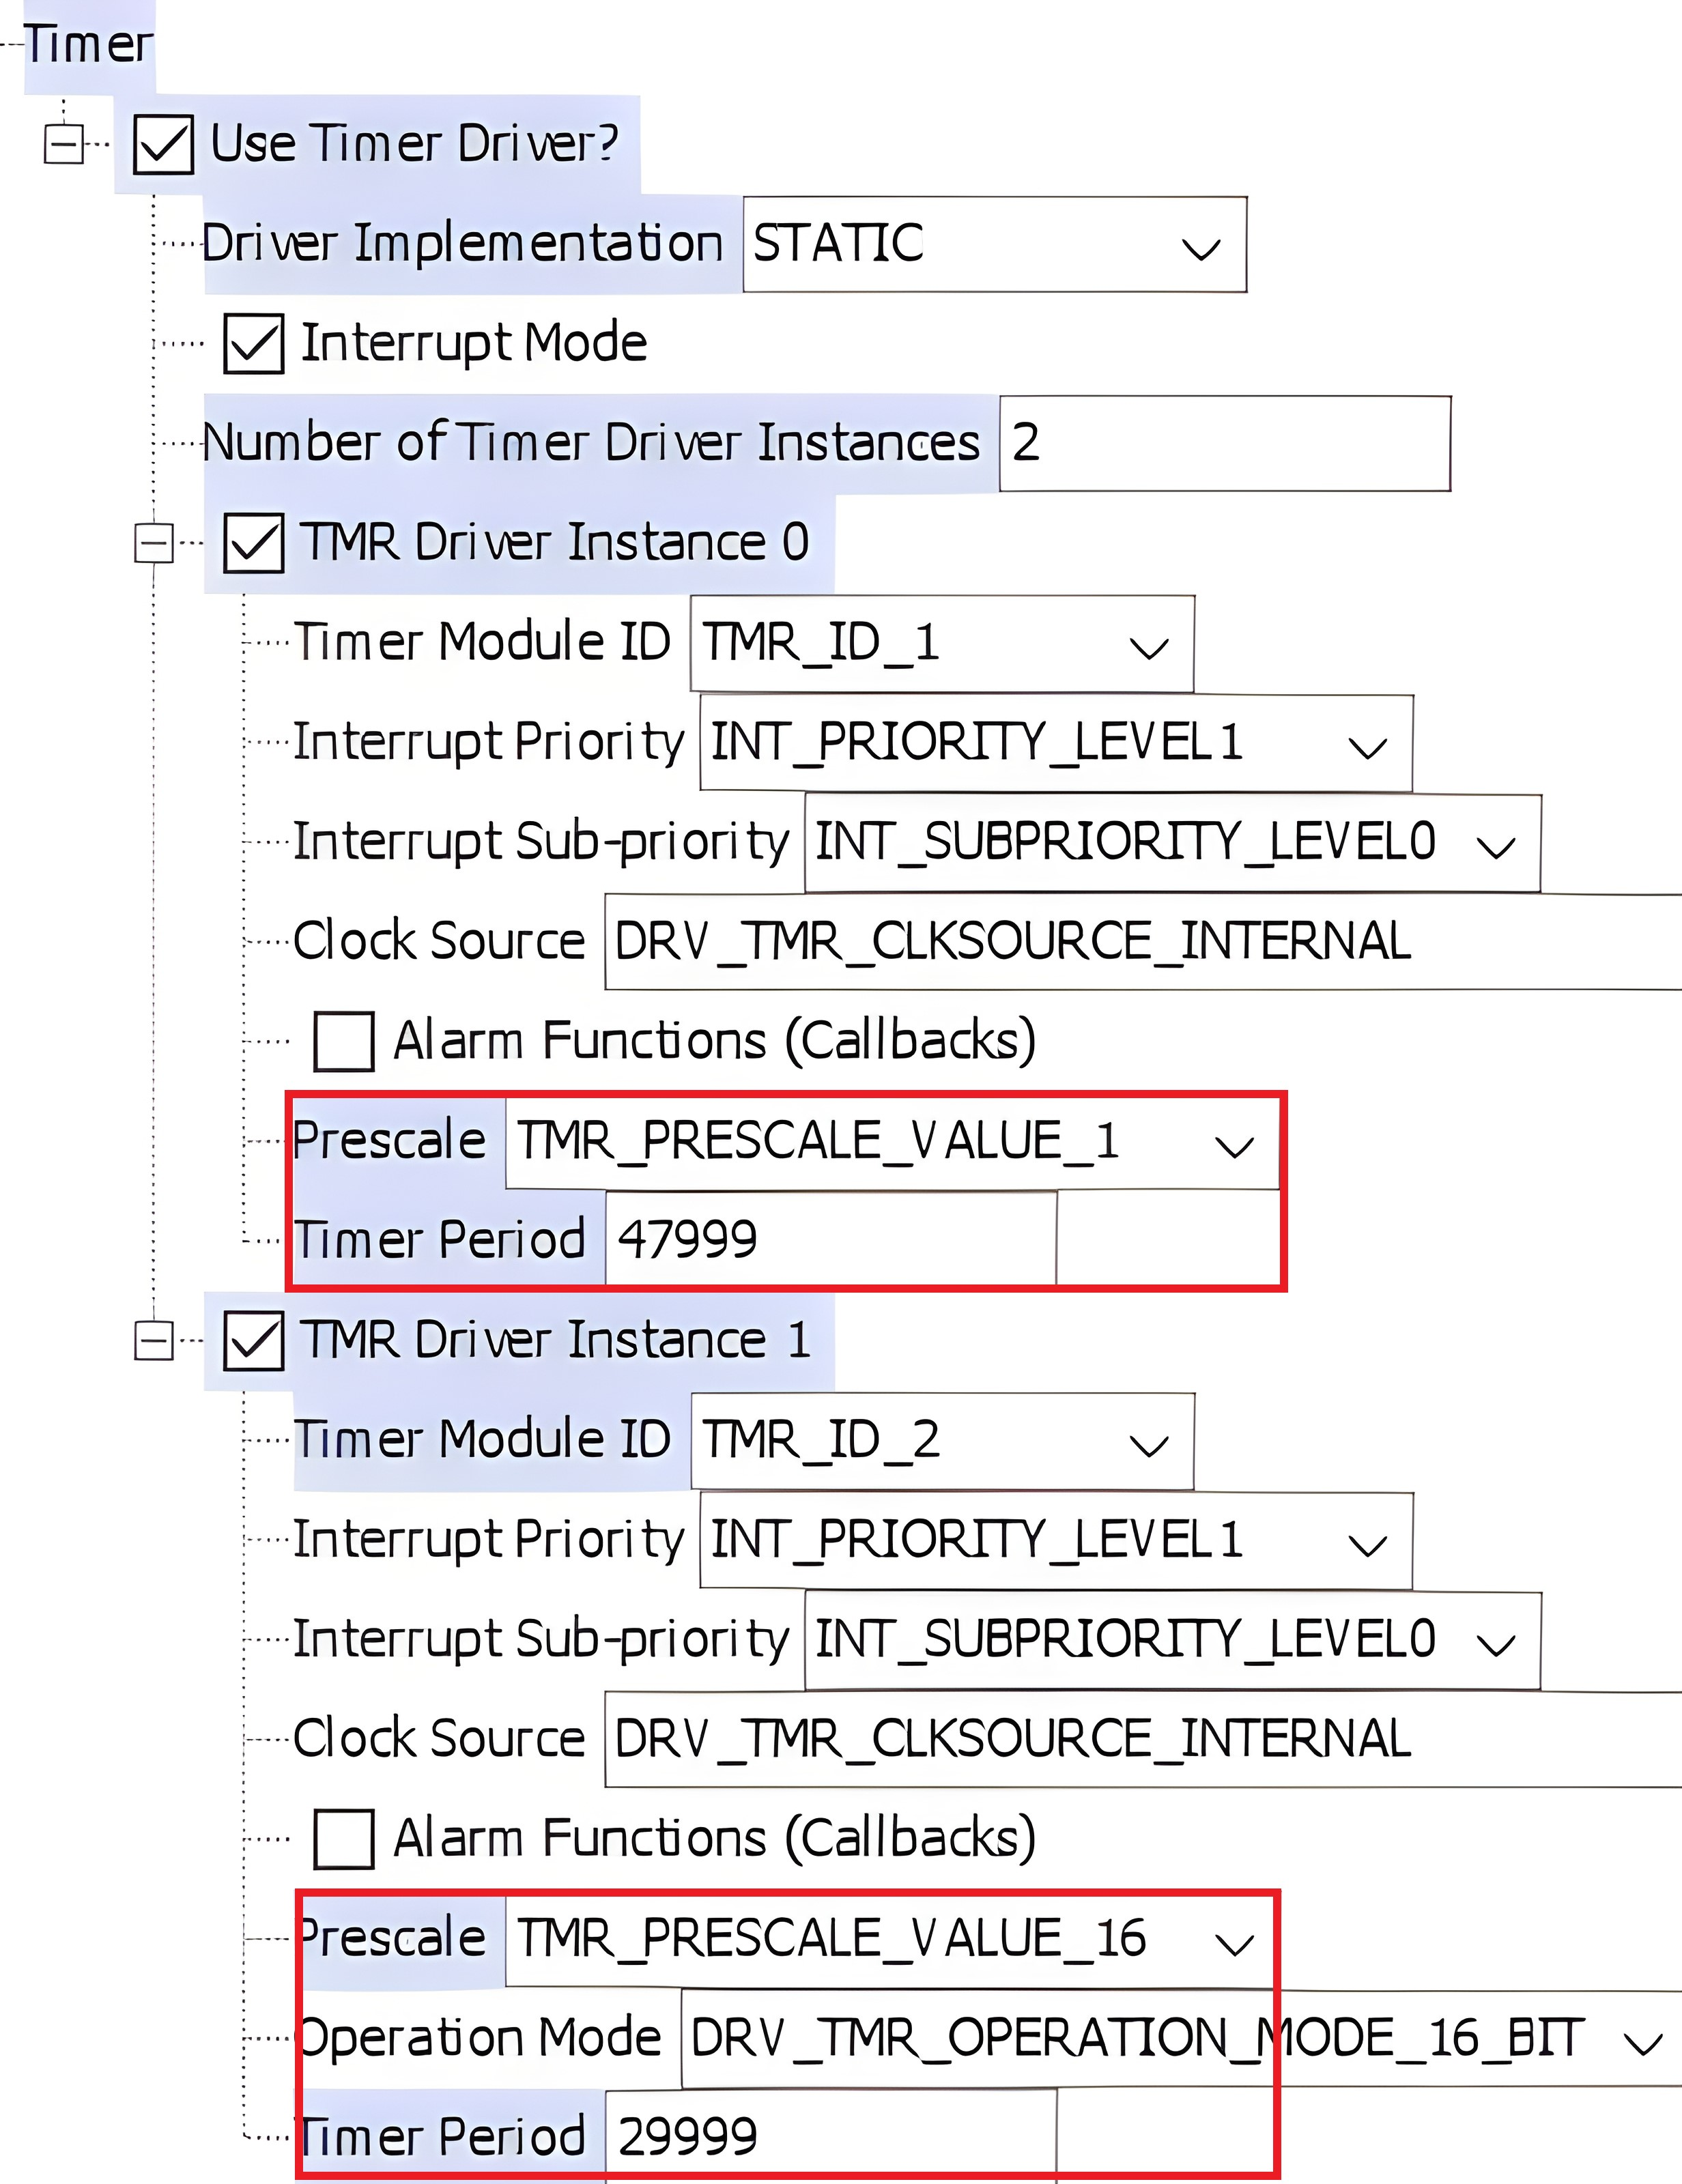
\includegraphics[width=.5\linewidth]{../figures/code/harmony/timers}}
	\caption{Configuration des timers.}
	\source{Auteur}
	\label{fig:timers}
\end{figure}

\clearpage

\begin{code}
\caption{Interruption \textbf{timer 1}, 1 [$ms$]}
\label{code:int-t1}
\begin{minted}[breaklines]{c}
void delayTimer_callback(){
	/* Increment delay timer */
	timeData.delayCnt ++;
}
\end{minted}
\end{code}

\begin{code}
\caption{Interruption \textbf{timer 2}, 10 [$ms$]}
\label{code:int-t2}
\begin{minted}[breaklines]{c}
void stateTimer_callback()
{
	/* Increment all counters */
	timeData.ledCnt ++;
	timeData.measCnt[BNO055_idx] ++;
	timeData.measCnt[GNSS_idx] ++;
	timeData.tmrTickFlag = true;
	/* When the button is pressed, the hold time is counted. */
	if(timeData.flagCntBtnPressed){
		timeData.cntBtnPressed++;
	}
	/* Do debounce on button every 10 ms */
	DoDebounce(&switchDescr, ButtonMFStateGet());
	/* Start a measure set each IMU period */        
	if ( ( timeData.measCnt[BNO055_idx] % (timeData.measPeriod[BNO055_idx]/10) ) == 0)
	timeData.measTodo[BNO055_idx] = true;
	
	/* Start a measure set each GNSS period */        
	if ( ( timeData.measCnt[GNSS_idx] % (timeData.measPeriod[GNSS_idx]/10) ) == 0)
	timeData.measTodo[GNSS_idx] = true;
	/* Manage LED if enabled */
	if((timeData.ledCnt >= LED_PERIOD) && (appData.ledState == true))
	LED_BOff();
} 
\end{minted}
\end{code}	

Dans le code \ref{code:int-t2}, nous pouvons voir le code de la routine d'interruption du timer 2. Lors de cette interruption, les différents compteurs de mesures sont incrémentés et différentes conditions vont tester si la période de mesure est atteinte. Une gestion du bouton a également lieu, notamment une mesure du temps d'appui, et une limitation des effets de rebonds mécaniques sur les signaux électriques observés par le \gls{mcu} par un échantillonnage diminué. Enfin, la LED de vie est gérée, notamment son temps allumé.


\clearpage

\subsection{Application principale} 

Lors de cette section nous allons décrire le fonctionnement principale du système sous la forme d'un diagramme d'état sur la figure \ref{fig:stateapp}.

\begin{figure}[h]
	\centering
	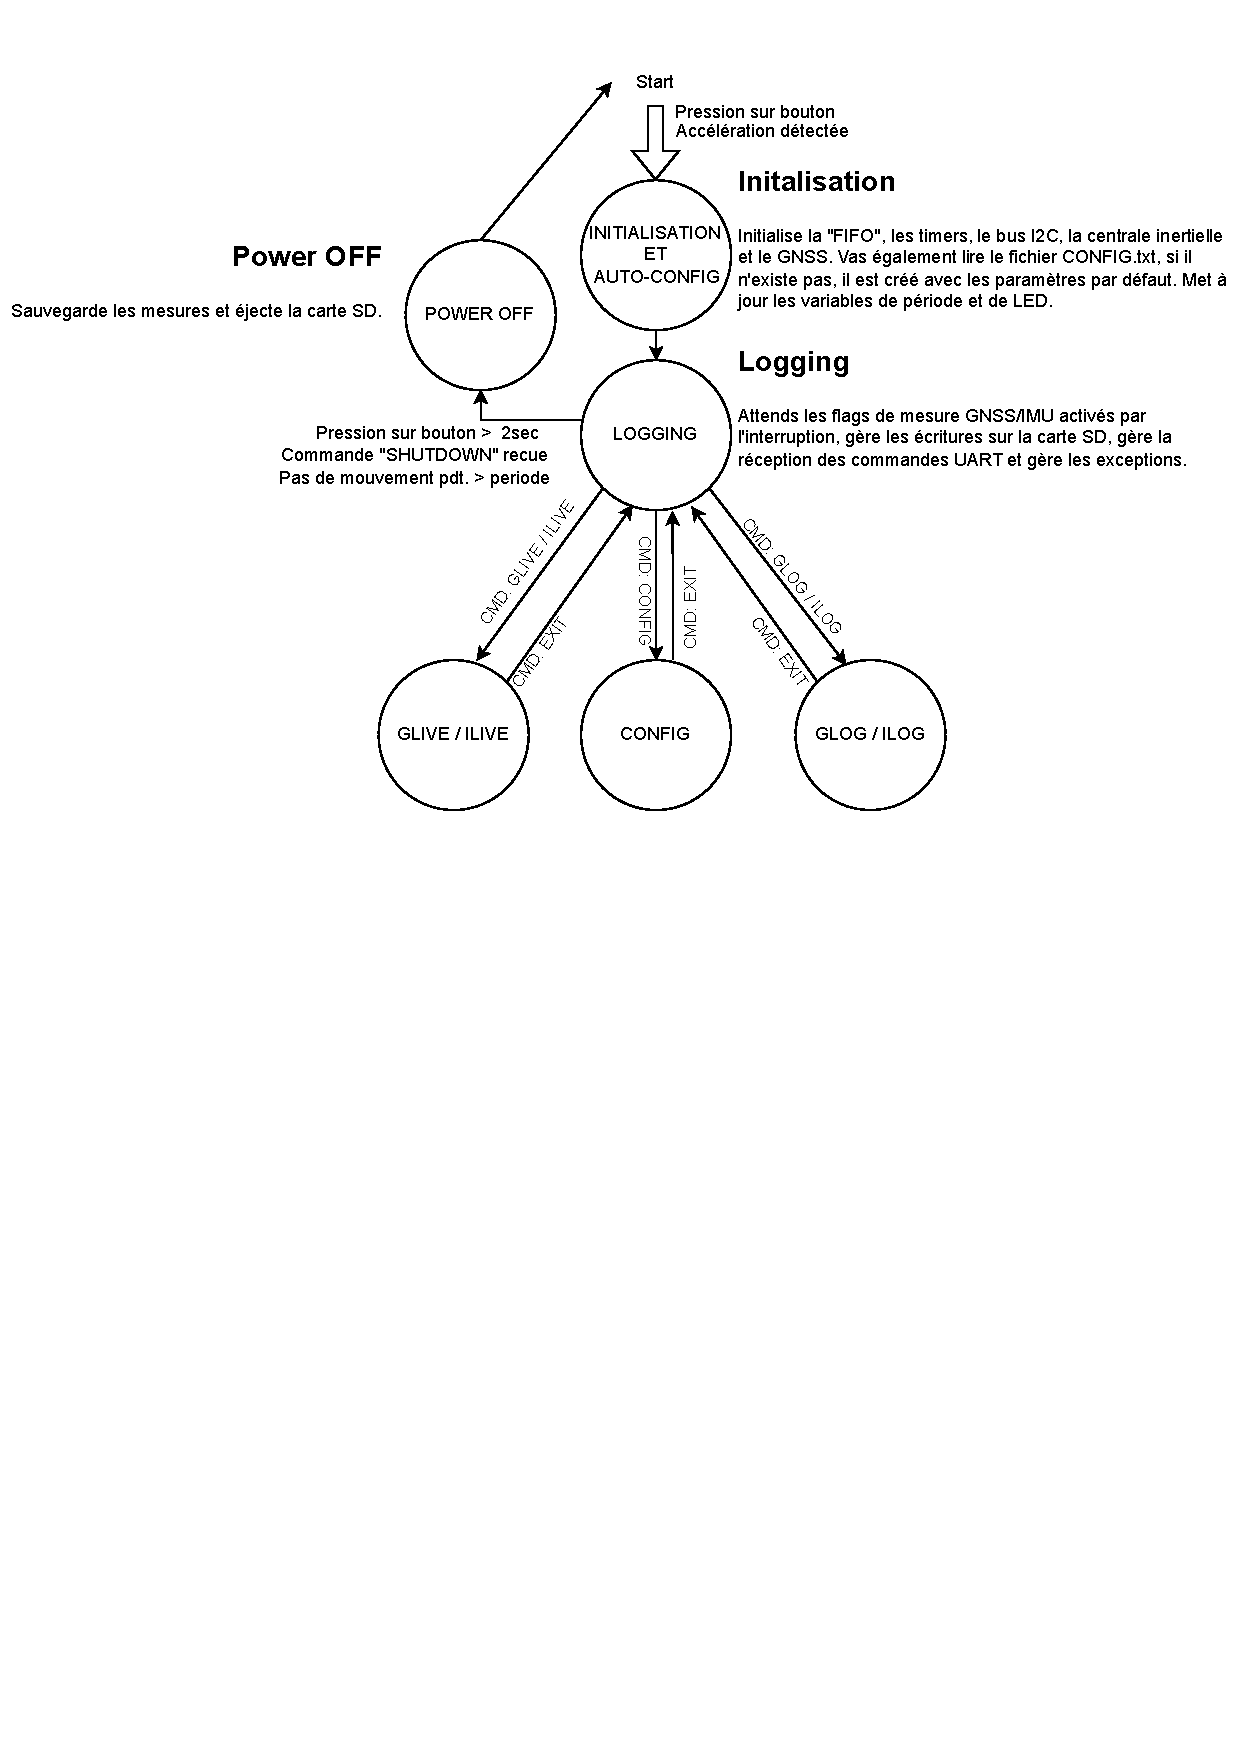
\includegraphics[width=1\linewidth]{../figures/code/diagrammes/state_app}
	\caption{Diagramme d'état principal.}
	\label{fig:stateapp}
	\source{Auteur}
\end{figure}

\subsubsection{Commandes USB-UART}
Les commandes permettent d'interagir avec le système et de manipuler les différentes données de la boîte noire.

\begin{center}
	\underline{Liste des commandes}
	\begin{table}[h]
		\centering
		\resizebox{\textwidth}{!}{
			\begin{tabular}{llll}
			GLIVE & -LVG & : & Permet d'afficher les données du \gls{gnss} en live sur le terminal sans les enregistrer. \\
			ILIVE & -LVI & : & Lance l'envoi des données live de l'\gls{imu} sans les enregistrer. \\
			GLOG & -GL & : & Envoie les données de localisation de la carte-SD au terminal. \\
			ILOG & -IL & : & Envoie les données inertielle de la carte-SD au terminal.\\
			GCLR & -GC & : & Supprime les logs du \gls{gnss}.\\
			ICLR & -IC & : & Supprime les logs de l'\gls{imu}.\\
			EXIT & X & : & Quitte le mode en cours.\\
			SHUTDOWN & -OFF & : & Sauvegarde et éteint le système. \\
			CONFIG & -CFG & : & Démarre le mode de configuration du système. \\
			\faChevronRight & INTG:XXXX & : & Dans mode config. permet de régler la période de mesure du \gls{gnss}.\\
			\faChevronRight & INTI:XXXX & : & Dans mode config. permet de régler la période de mesure de l'\gls{imu}. \\
			\faChevronRight & LEDV:X & : & Dans mode config. permet d'activer ou non la LED de vie. \\
			\faChevronRight & TOFF:XX & : & Dans mode config. permet de fixer le temps d'inactivité (éteint le système).
		\end{tabular}
		}
		\caption{Commandes disponibles}
		\label{tab:cmdDisp}
	\end{table}
\end{center}

Les commande de la table \ref{tab:cmdDisp} peuvent également être envoyés en caractères minuscules.

\clearpage

Sur la figure \ref{fig:sequence-app}, la séquence de la boucle principale de l'application est représentée. Celle-ci interagit avec les différents périphériques en utilisant diverses bibliothèques C.

\begin{figure}[!h]
	\centering
	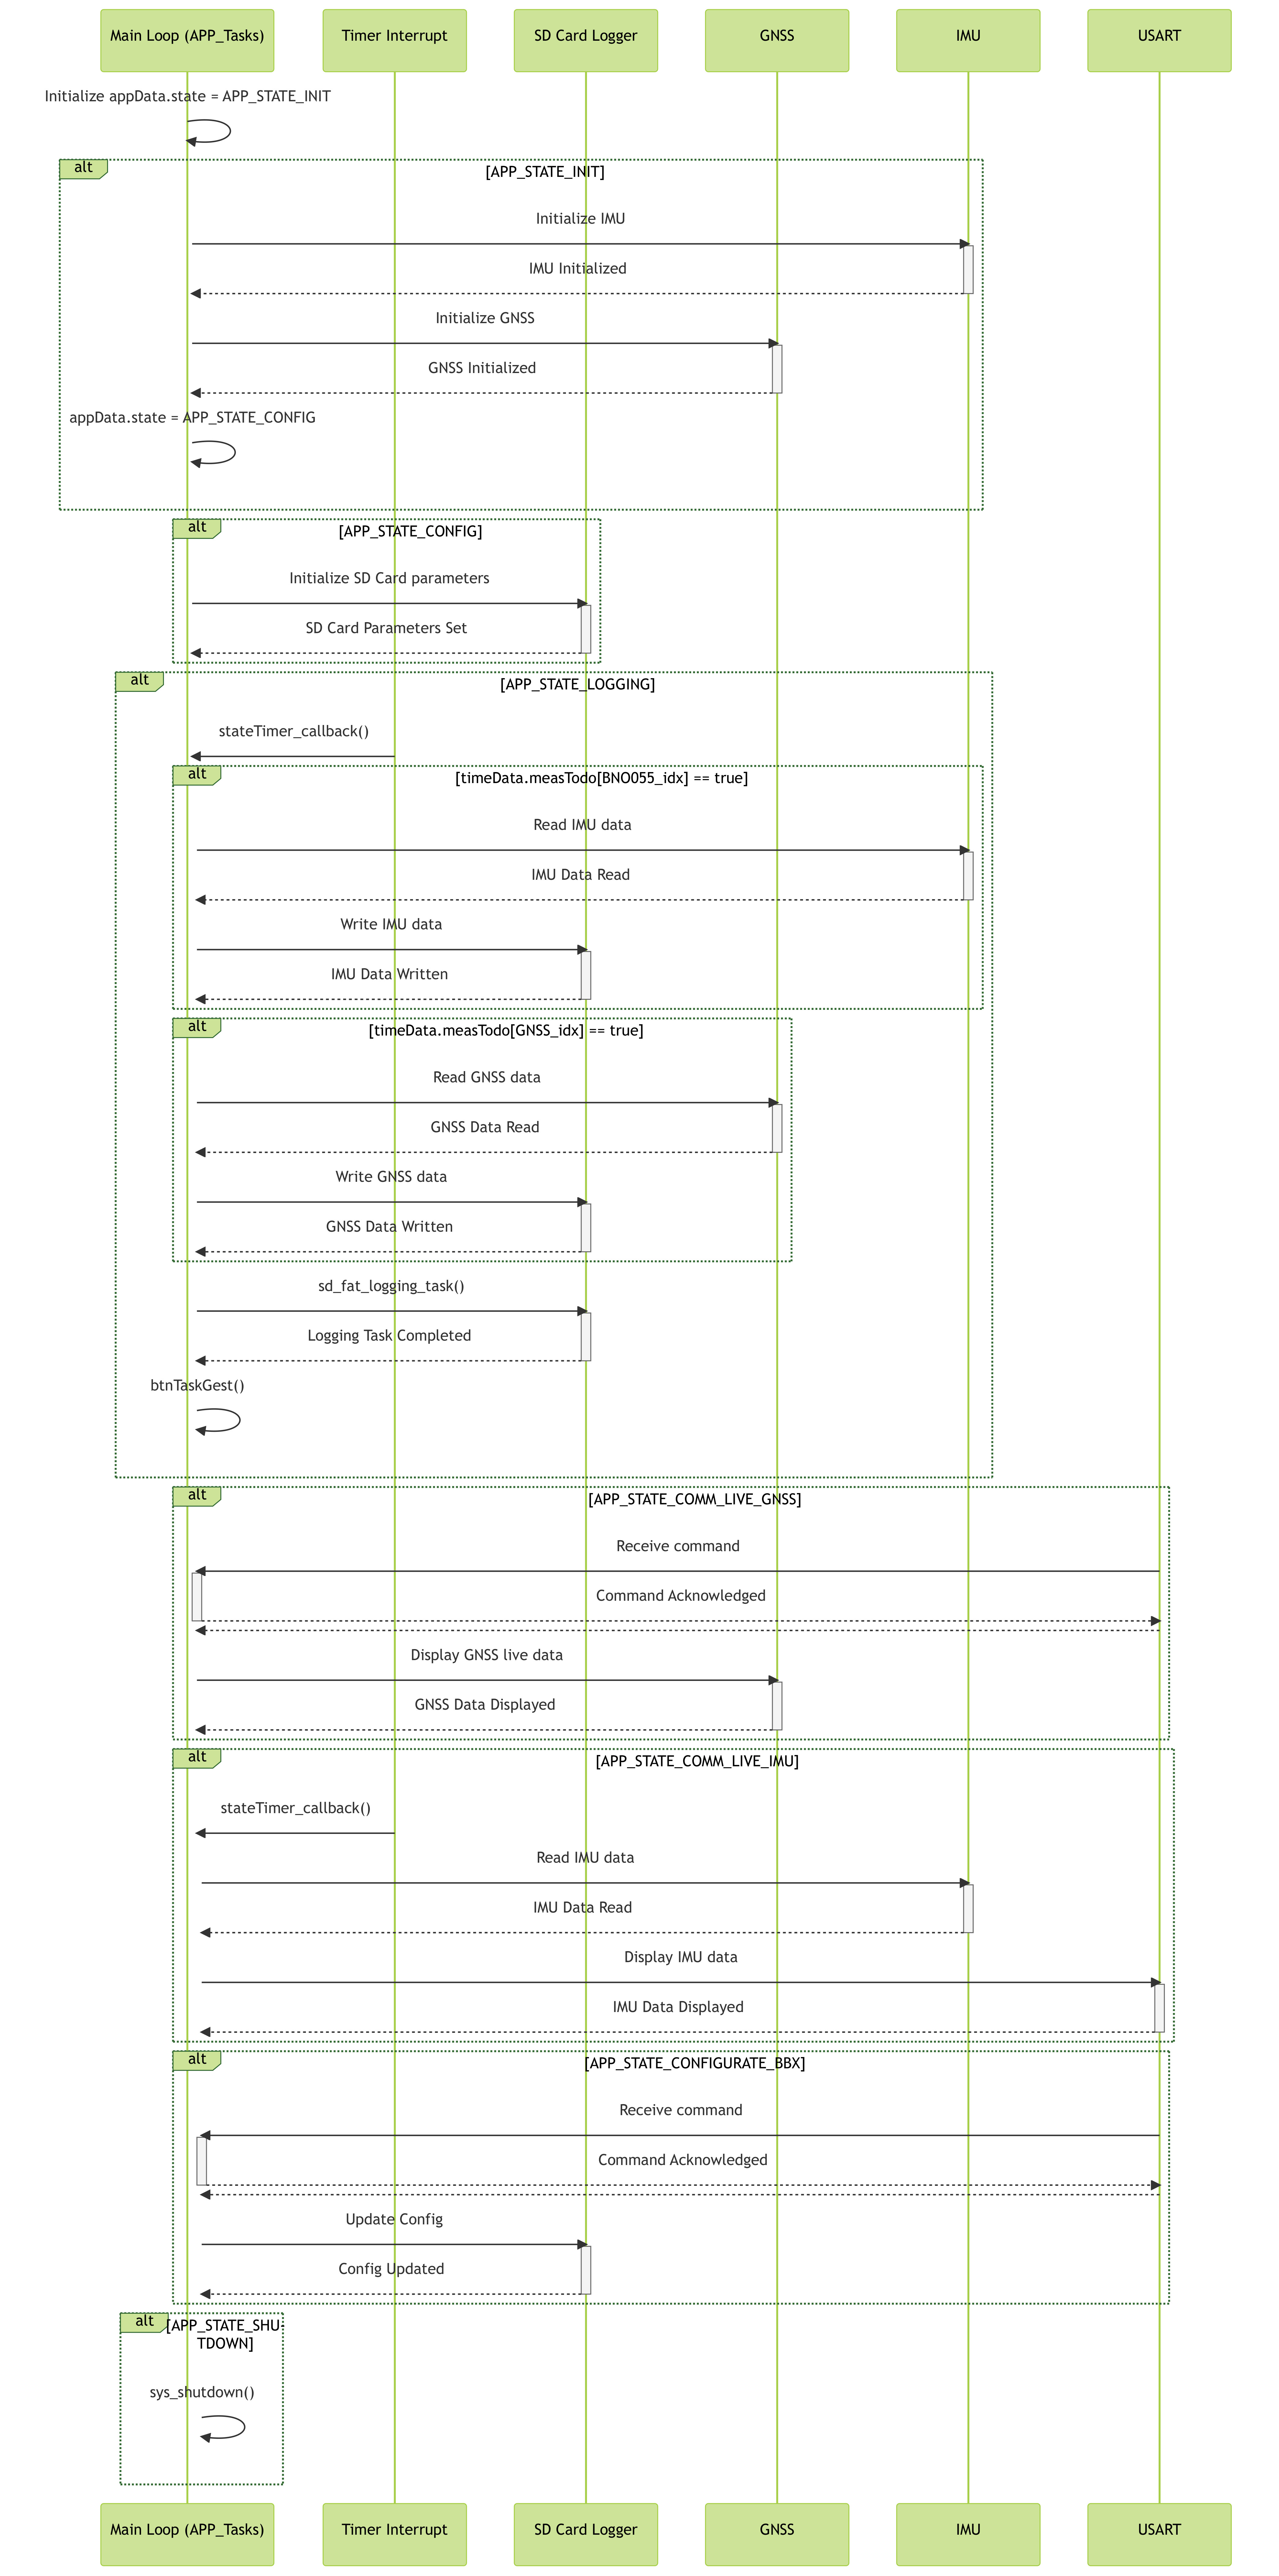
\includegraphics[width=.65\linewidth]{../figures/code/diagrammes/sequence-app}
	\caption{Diagramme de séquence principal.}
	\label{fig:sequence-app}
	\source{Auteur}
\end{figure}

